\section{An Empirical Study of RL Scaling}
\label{sec:experiments}



In this section, we conduct RL experiments using an 8B dense model on verifiable math problems. Using the setup described in \Cref{sec:methodology}, we study several design axes in terms of their predictable compute-scaling behavior, namely \emph{asymptotic performance}~($A$) and \emph{compute efficiency}~($B$), as shown in \Cref{fig:interpreting_fit}.  

We structure our experiments in three stages -- we first ablate design choices on top of the baseline at $3.5k$ to $4k$ GPU-hours since some experimental choices destabilize beyond this scale~(Appendix~\ref{appendix:truncations}). Whenever a design change proved stable, we trained it for longer. Then, we combine the best choices into \scalerl\ and run leave-one-out (LOO) experiments for $16k$ GPU-hours in \Cref{sec:loo}. Here, we assess predictability by fitting on the first $8k$ GPU-hours and extrapolating the remainder of the run.  Finally, to demonstrate predictable scaling with \scalerl, we also consider training setups with larger batch sizes, mixture-of-experts model, multiple tasks (math and code), and longer sequence lengths in~\Cref{sec:diff_axes}.




\subsection{Asynchronous RL Setup} \label{sec:infra}

\begin{figure*}[t]
    \centering
    \subfloat[][]{
        \centering
        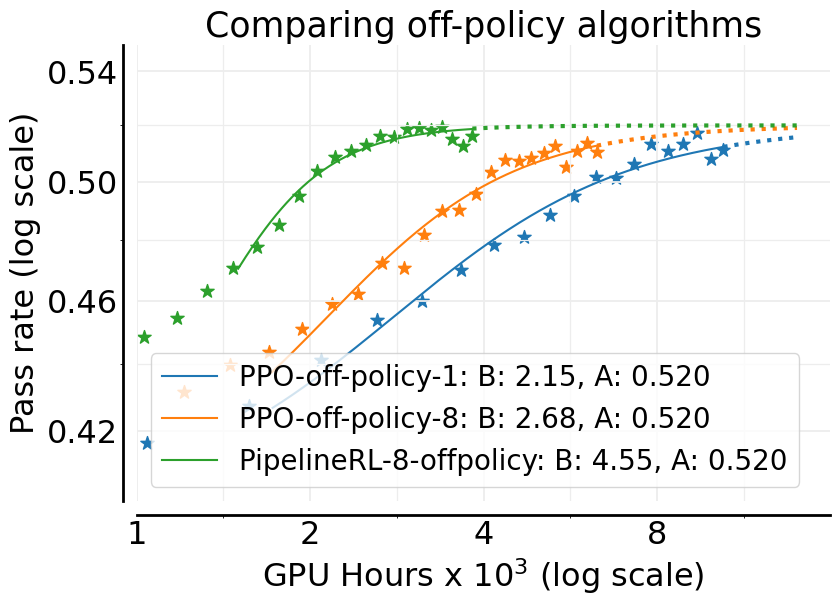
\includegraphics[width=0.45\textwidth]{paper_figs/infra.png}
        \label{fig:rl_infra}}
    \subfloat[][]{
        \centering
        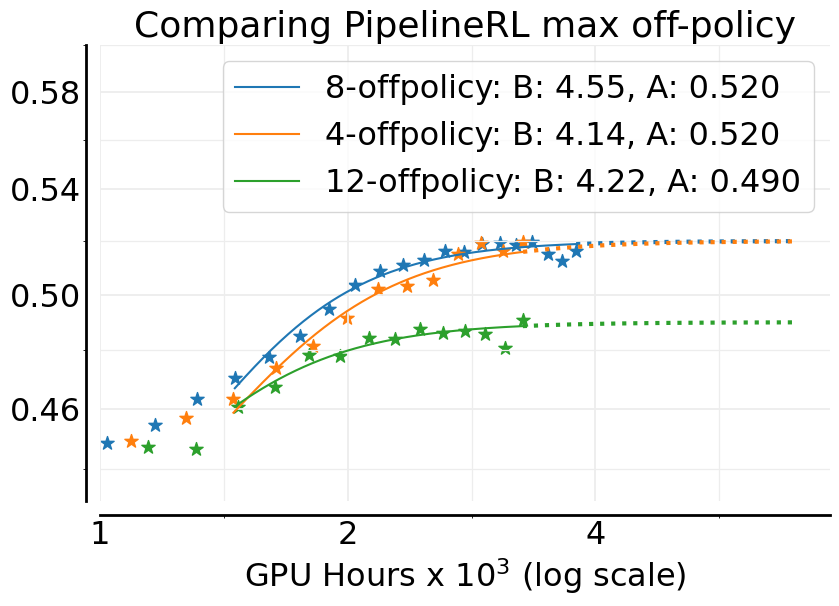
\includegraphics[width=0.45\textwidth]{paper_figs/pipelinerl_max_offpolicy.png}
        \label{fig:pipelinerl_offpolicy_app}}
    \caption{\small (a) \textbf{Comparing ``compute-scaling'' of asynchronous off-policy RL setups}. We report only the $B$ (scaling exponent) and $A$ (asymptotic pass rate) parameters of the fitted sigmoid curve (Equation~\ref{eq:sigmoid_law}). PipelineRL-$k$ is much more efficient and slightly better in the large compute limit. (b) \textbf{Different max off-policyness} with PipelineRL.}
\end{figure*}

We first investigate the choice of asynchronous off-policy RL setup~\citep{noukhovitch2024asynchronous}, as it governs training stability and efficiency, generally independent of all other design choices. Specifically, we consider two approaches for off-policy learning: PPO-off-policy-$k$ and PipelineRL-$k$. 



\textbf{PPO-off-policy-$k$} is the default approach for asynchronous RL and has been used previously by Qwen3~\citep{qwen3technicalreport} and ProRL~\citep{prorl}. In this setup, the old policy $\pi_{gen}^{\theta_{\text{old}}}$ generates reasoning traces for a batch of $B$ prompts. 
Each gradient update processes a mini-batch of $\hat{B}$ prompts, resulting in $k = B / \hat{B}$ gradient updates per batch. 
In our experiments, we fix $\hat{B}=48$ prompts (with 16 generations each), and vary $k \in \{1,8\}$ by setting $B = k \times 48$. 

\textbf{PipelineRL-$k$} is a recent approach from \citet{pipelinerl} and used by Magistral~\citep{rastogi2025magistral}. In this regimen, generators continuously produce reasoning traces in a streaming fashion. Whenever trainers finish a policy update, the new parameters are immediately pushed to the generators, which continue generating with the updated weights but a stale KV cache from the old policy. 
Once a full batch of traces is generated, it is passed to the trainers for the next update. 
In our setup we introduce a parameter $k$: the trainers wait if they get $k$ steps ahead of the generators.



\begin{figure*}[t]
    \centering
    \subfloat[]{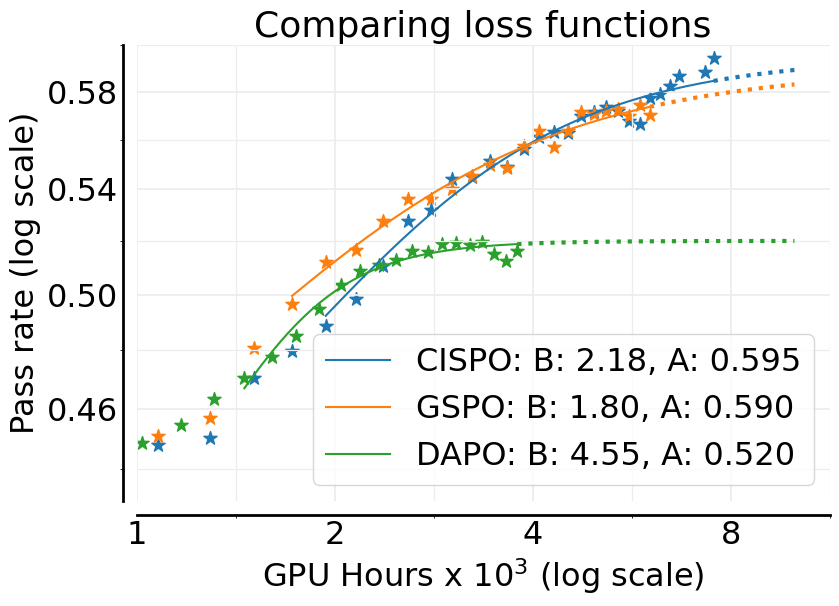
\includegraphics[width=0.45\textwidth]{paper_figs/loss_type.png} \label{fig:loss_type}} 
    ~~
    \subfloat[]{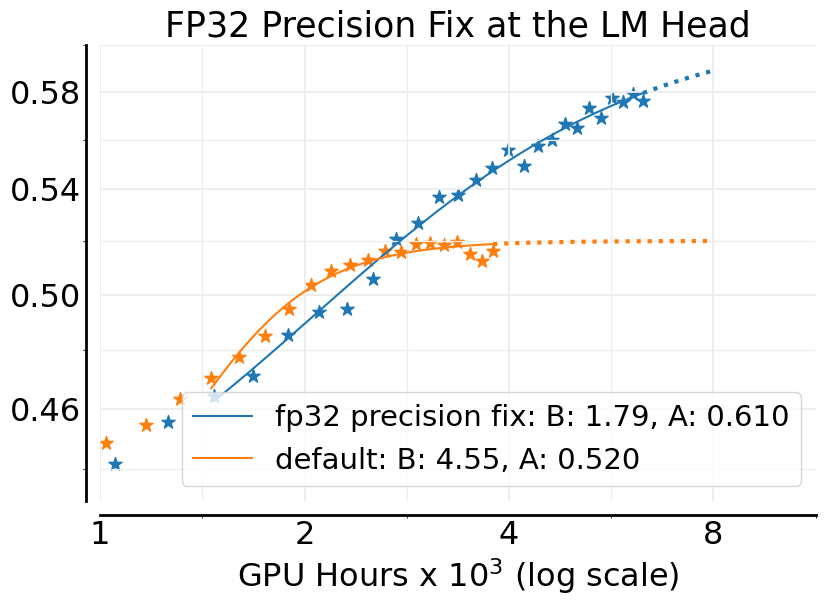
\includegraphics[width=0.45\textwidth]{paper_figs/fp32.png} \label{fig:fp32}}
    % \hfill
    % \subfloat[]{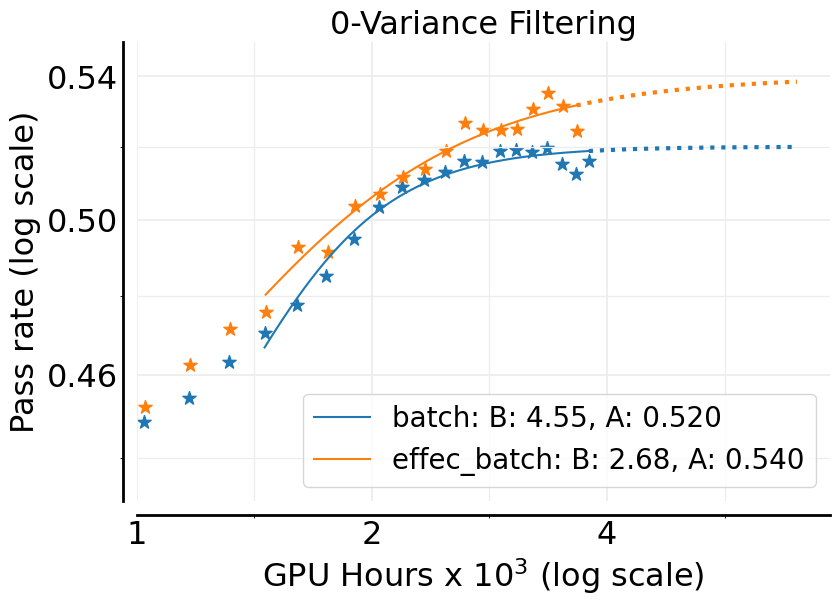
\includegraphics[width=0.45\textwidth]{paper_figs/0var_filtering.png} \label{fig:0var_main}} 
    % ~~
    % \subfloat[]{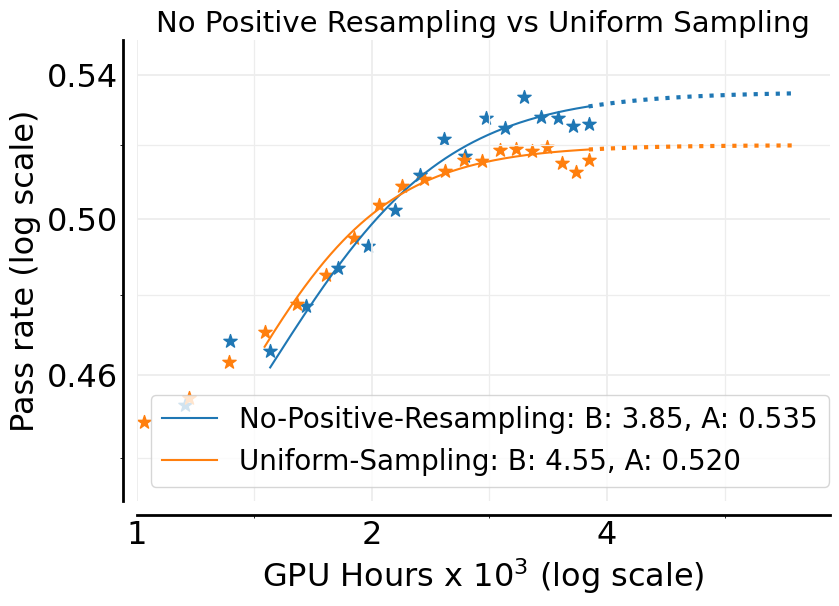
\includegraphics[width=0.45\textwidth]{paper_figs/noposresample.png} \label{fig:nopos_main}} 
    \caption{\small (a) \textbf{Comparing popular loss functions}: DAPO \citep{yu2025dapo}, GSPO \citep{gspo}, and CISPO \citep{minimax_m1}. We find CISPO/GSPO achieve a higher asymptotic reward compared to DAPO. (b) \textbf{Using FP32 precision} in the final layer (LM head) gives a considerable boost in the asymptotic reward.}\label{main:filter}
\end{figure*}

\begin{figure*}[t]
    \centering 
    \subfloat[]{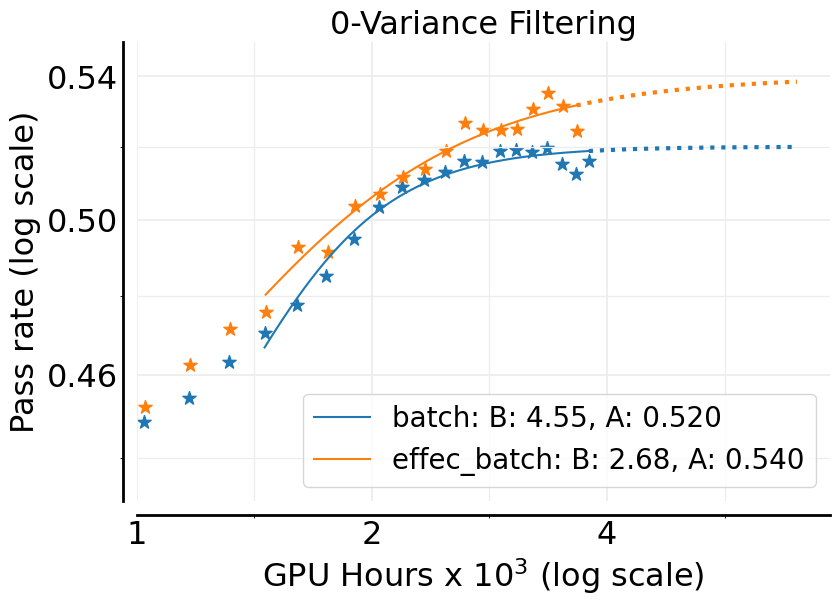
\includegraphics[width=0.45\textwidth]{paper_figs/0var_filtering.png} \label{fig:0var_main}} 
    ~~
    \subfloat[]{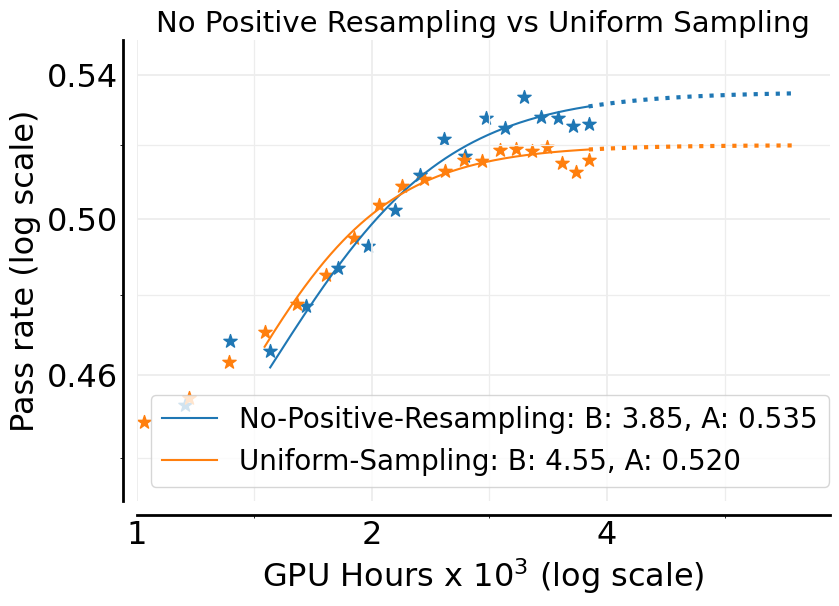
\includegraphics[width=0.45\textwidth]{paper_figs/noposresample.png} \label{fig:nopos_main}} 
    \caption{\small (a) \textbf{``Zero'' variance filtering:} We filter out ``zero'' variance (accuracy 0 or 1) samples in a batch since they contribute zero policy gradient and find it achieves a higher asymptote, and (b) \textbf{Adaptive prompt sampling:} Filtering out prompts with pass rate $\geq 0.9$ in subsequent epochs results in a higher asymptotic performance.}\label{main:filter}
\end{figure*}

We compare these approaches in \Cref{fig:rl_infra}. 
PipelineRL and PPO-off-policy achieve similar asymptotic performance $A$, but PipelineRL substantially improves the compute efficiency $B$; thus reaching the ceiling $A$ faster. This is because PipelineRL reduces the amount of idle time in the training process. This choice yields reliable gains with fewer tokens, making larger sweeps at a lower compute budget possible. We also vary the maximum off-policyness for PipelineRL and find $k=8$ to be optimal as shown in \Cref{fig:pipelinerl_offpolicy_app}, which we discuss further in Appendix~\ref{appendix:pipelinerl}.

\subsection{Algorithmic Choices} \label{sec:fwd_ablations}
Building on the results above, we adopt PipelineRL-$8$ as our updated baseline. 
We then study six additional algorithmic axes: (a) loss aggregation, (b) advantage normalization, (c) precision fixes, (d) data curriculum, (e) batch definition, and (f) loss type. In \Cref{sec:loo}, we combine the best options into a unified recipe, termed \scalerl (\textbf{Scale}-able \textbf{RL}), and conduct leave-one-out experiments on a larger scale of $16,000$ GPU-Hours.

\paragraph{Loss type}
\phantomsection
\label{sec:loss_type}

We compare the asymmetric DAPO loss~(Eq.~\ref{eq:dapo_loss}) with two recently proposed alternatives: GSPO~\citep{gspo} and CISPO~\citep{minimax_m1, feng2025yourefficient}. GSPO applies importance sampling at the sequence level as opposed to GRPO’s token-level formulation. Specifically, GSPO alters the token-level IS ratio (Eq.~\ref{eq:is}) to sequence-level ratios: $ \rho_i(\theta) = \nicefrac{\pi_{train}(y_i|x, \theta)}{\pi_{gen}(y_i|x, \theta_{\text{old}})}$. CISPO simply combines truncated IS with vanilla policy gradient~\citep{ionides2008truncated}, where $\texttt{sg}$ is the stop-gradient function:
\begin{equation}
\hspace{-0.7em} \mathcal{J}_{\mathrm{CISPO}}(\theta) 
=\hspace{-0.7em} \underset{\substack{x \sim D, \\ \{y_i\}_{i=1}^G \sim \pi_{gen}(\cdot \mid x, \theta_{\text{old}})}}{\mathbb{E}}
% = \mathbb{E}_{\begin{subarray}{l} \, x \sim D, \\ \{y_i\}_{i=1}^G \sim \pi_{\text{gen}(\cdot \mid x, \theta_{\text{old}})} \end{subarray}}
\hspace{-0.4em}
\left[ \frac{1}{T} \sum_{i=1}^G \sum_{t=1}^{|y_i|} 
\texttt{sg}(\mathrm{min}(\rho_{i, t}, \epsilon_\text{max})) 
\hat{A}_i \, \log\left(\pi_{train}(y_{i,t}|x, y_{i<t},\theta)\right) \right]
\label{eq:cispo}
\end{equation} 


Figure~\ref{fig:loss_type} shows that both GSPO and CISPO substantially outperform DAPO, improving the asymptotic pass-rate $A$ by a large margin. CISPO exhibits a prolonged near-linear reward increase, and is marginally better than GSPO later in training, so we opt for CISPO as our best loss type. Further discussion on off-policy loss types, and their hyperparameter robustness is detailed in \Cref{sec:loo} and Appendix~\ref{appendix:loss_types}.



\paragraph{FP32 Precision for LLM logits}
\phantomsection
\label{sec:fp32}

The generators and trainers rely on different kernels for inference and training, leading to small numerical mismatches in their token probabilities~\citep{he2025nondeterminism}. 
RL training is highly sensitive to such discrepancies, since they directly affect the IS ratio in the surrogate objective.
\citet{minimax_m1} identified that these mismatches are especially pronounced at the language model head, and mitigate this by FP32 computations at the head for both the generator and trainer. 
As shown in \Cref{fig:fp32}, the precision fix dramatically improves the asymptotic performance $A$ from $0.52$ to $0.61$. Given this clear benefit, we include the FP32 precision fix in our \scalerl\ recipe. 



\paragraph{Loss Aggregation}

We evaluate three strategies for aggregating the RL loss: (a) \emph{Sample average} where each rollout contributes equally (as in GRPO, Appendix~\ref{appendix:background}). (b) \emph{Prompt average} where each prompt contributes equally (as in DAPO, Appendix~\ref{appendix:background}). (c) \emph{Token average} where all token losses in the batch are averaged directly, without intermediate grouping. The comparison results are shown in Appendix~\ref{appendix:forward} (\Cref{fig:loss_agg}).
We find prompt-average achieves the highest asymptotic performance and therefore use this choice for \scalerl. 


\paragraph{Advantage Normalization}

We compare three variants of advantage normalization: (a) \emph{Prompt level} where advantages are normalized by the standard deviation of rewards from the rollouts of the same prompt (as in GRPO, Appendix~\ref{appendix:background}). (b) \emph{Batch level} where advantages are normalized by the standard deviation across all generations in the batch, as used by \citet{hu2025reinforce_pp,rastogi2025magistral}. (c) \emph{No normalization} where advantages are computed as raw rewards centered by the mean reward of the prompt’s generations, without variance scaling (as proposed in Dr.\ GRPO~\citep{dr_grpo}). A comparison plot is shown in Appendix~\ref{appendix:forward} (\Cref{fig:adv_norm}), and all three methods are oberseved to yield similar performance. We therefore adopt batch-level normalization as it is theoretically sound and marginally better. This choice is also further corroborated at a larger scale by the leave-one-out experiments in \Cref{sec:loo}.

\paragraph{Zero-Variance Filtering}
\phantomsection
\label{sec:batch_definition}

Within each batch, some prompts yield identical rewards across all their generations. 
These ``zero-variance'' prompts have zero advantage and therefore contribute zero policy gradient. 
The default baseline includes such prompts in loss computation, but it is unclear whether they should be included in the effective batch. 
To test this, we compare the default setting against an \emph{effective batch} approach, where only prompts with non-zero variance are included in the loss calculation, as done by \citet{seed2025seed1}. Note that zero-variance filtering differs from dynamic sampling in DAPO~\citep{yu2025dapo}. The former merely drop the prompts, while latter resamples more prompts until the batch is full.
We show in \Cref{fig:0var_main} that using the effective batch performs better asymptotically; and we adopt it in our \scalerl\ recipe.

\paragraph{Adaptive Prompt Filtering}

A number of data curriculum strategies have been proposed for RL training to improve sample efficiency~\citep{polaris2025,speedrl,greso}. Here we evaluate a simple variant, introduced by \citet{polaris2025}, with the key observation that once a prompt becomes too easy for a policy, it typically remains easy.
Since such prompts consume some compute but no longer contribute useful gradient signal (\Cref{sec:batch_definition}), it is better to exclude them from future training. 
We implement this by maintaining a history of pass rates and permanently removing any prompt with pass rate $\geq 0.9$ from subsequent epochs--we call this \textbf{No-Positive-Resampling}.
In \Cref{fig:nopos_main} we compare this curriculum against the default setting where all prompts are resampled uniformly throughout training. 
We see that the curriculum improves scalability and the asymptotic reward $A$.

\section{\scalerl: Scaling RL Compute Effectively \& Predictably}
\label{sec:loo}





From the design axes studied above, we consolidate the best-performing settings into a single recipe, which we term \scalerl\ (\textbf{Scale}-able \textbf{RL}). 
\scalerl\ is an asynchronous RL recipe that uses \textbf{PipelineRL with $8$ steps off-policyness}, \textbf{interruption-based length control} for truncation, \textbf{FP32 computation for logits}, and optimizes the $\mathbf{\mathcal{J}_{\mathrm{\scalerl}}(\theta)}$ \textbf{loss}. This loss combines prompt-level loss aggregation, batch-level advantage normalization, \textbf{truncated importance-sampling} REINFORCE loss~(CISPO) , zero-variance filtering, and no-positive resampling: 
\begin{align*}
& \mathcal{J}_{\mathrm{\scalerl}}(\theta) 
=\hspace{-0.7em} \underset{\substack{x \sim D, \\ \{y_i\}_{i=1}^G \sim \pi_{gen}^{\theta_{old}}(\cdot \mid x)}}{\mathbb{E}}
\hspace{-0.4em}
\left[ \frac{1}{\sum_{g=1}^{G} |y_g|} \sum_{i=1}^G \sum_{t=1}^{|y_i|} \texttt{sg}(\mathrm{min}(\rho_{i, t}, \epsilon)) \hat{A}_{i}^{\text{norm}} \, \log\pi_{train}^\theta(y_{i,t})\right], \\
& \quad  \rho_{i, t}=\frac{\pi_{train}^\theta(y_{i,t})}{\pi_{gen}^{\theta_{old}}(y_{i,t})},\ \hat{A}^{\mathrm{norm}}_{i}
= \hat{A}_{i}/\hat{A}_{\text{std}},\ 0 <  \mathrm{mean}(\{r_j\}_{j=1}^G) < 1,\  \text{pass\_rate}(x) < 0.9,\ 
\end{align*}
where $\texttt{sg}$ is the stop-gradient function, $\hat{A}_{\text{std}}$ is the standard deviation of all advantages $\hat{A}_{i}$ in a batch and $\text{pass\_rate}(x)$ denotes the historical pass rate of a prompt $x$.  For forced interruptions, we use the end-of-thinking phrase: ``Okay, time is up. Let me stop thinking and formulate a final answer now. \texttt{</think>}''.


\paragraph{Leave-One-Out~(LOO) Ablations}
To validate that these choices remain optimal when combined, we conduct \emph{leave-one-out} (LOO) experiments: starting from \scalerl, we revert one axis at a time to its baseline counterpart from \Cref{sec:methodology}. 
This ensures that each design decision contributes positively even in the presence of all others. Figure~\ref{fig:LOO} reports these experiments, each scaled to $16$k GPU hours.

\begin{figure*}[t]
    \centering
    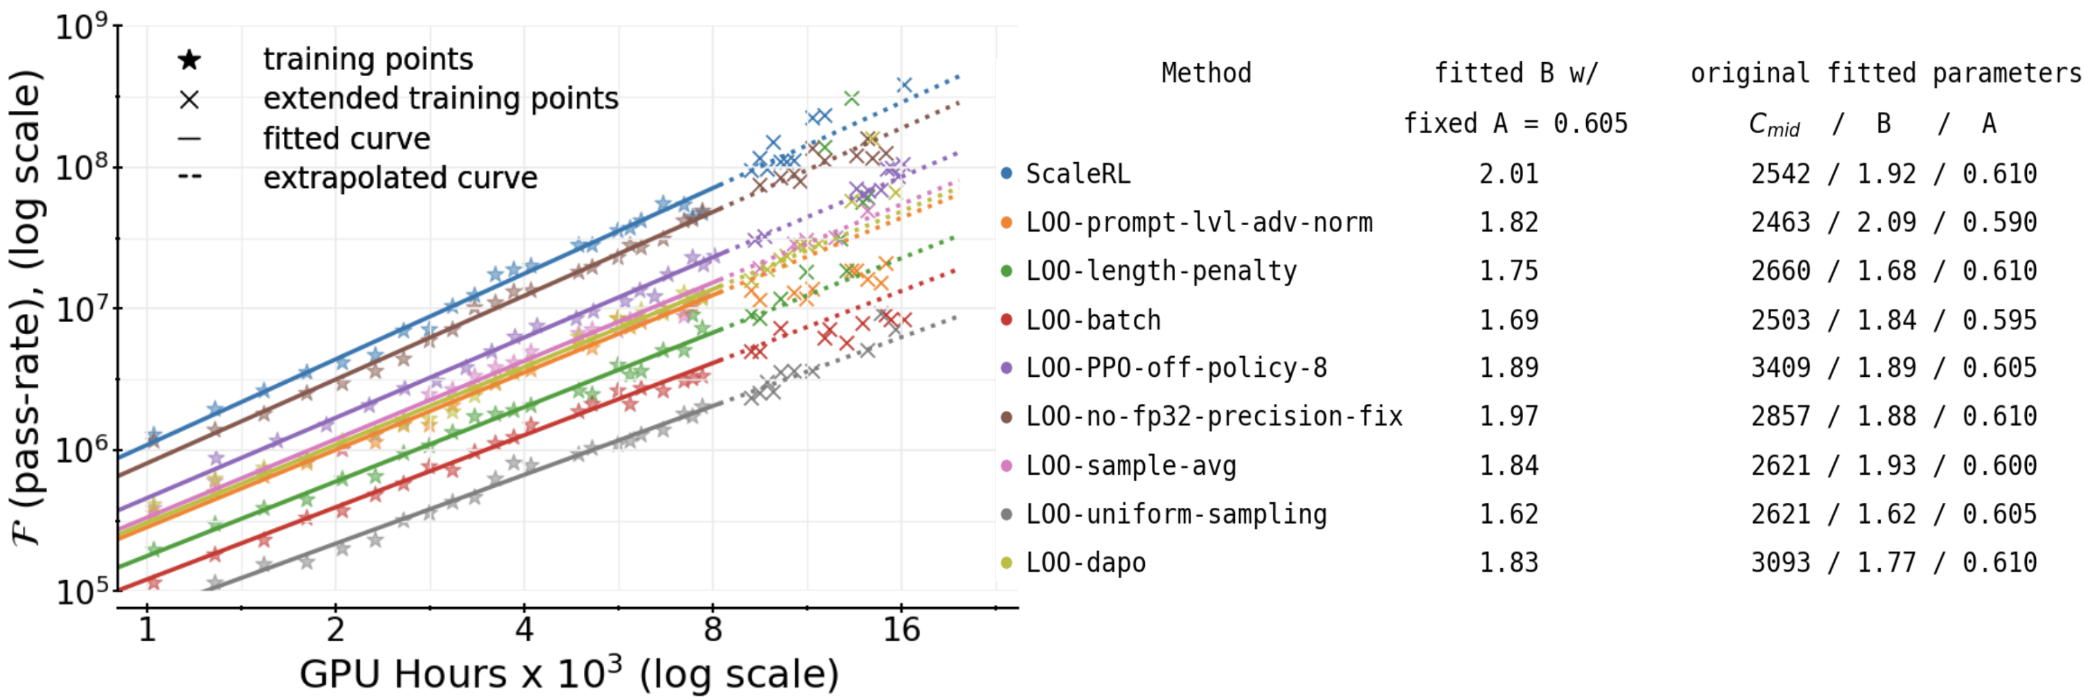
\includegraphics[width=1\textwidth]{paper_figs/LOO.png}
    \caption{\small{\textbf{Leave-One-Out (LOO) Experiments}: Starting from \scalerl, we revert one design choice at a time to its baseline counterpart and re-train. Most LOO variants reach a similar asymptotic reward, with \scalerl\ outperforming slightly overall. The main difference in these methods lies in efficiency. To highlight this, we re-arrange \Cref{eq:sigmoid_law} into $\mathcal{F}(R_c) = C^B$, where $\mathcal{F}(R_c) = C_{\text{mid}}^B / \big(\frac{A - R_0}{R_c - R_0} - 1\big)$, and plot $\log \mathcal{F}(R_c)$ vs. $\log C$. This form makes slope $B$ directly visible, showing that \scalerl\ achieves the highest compute efficiency.} 
    }
    \label{fig:LOO}
\end{figure*}




\begin{figure*}[t]
    \subfloat[]{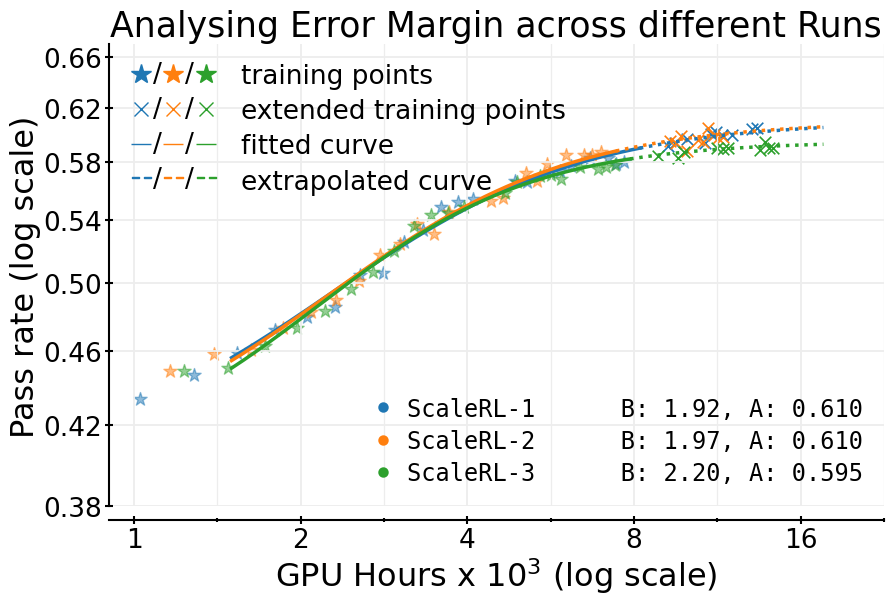
\includegraphics[width=0.49\textwidth]{paper_figs/error_margin.png} \label{fig:error_margin}}
    \hfill
    \subfloat[]{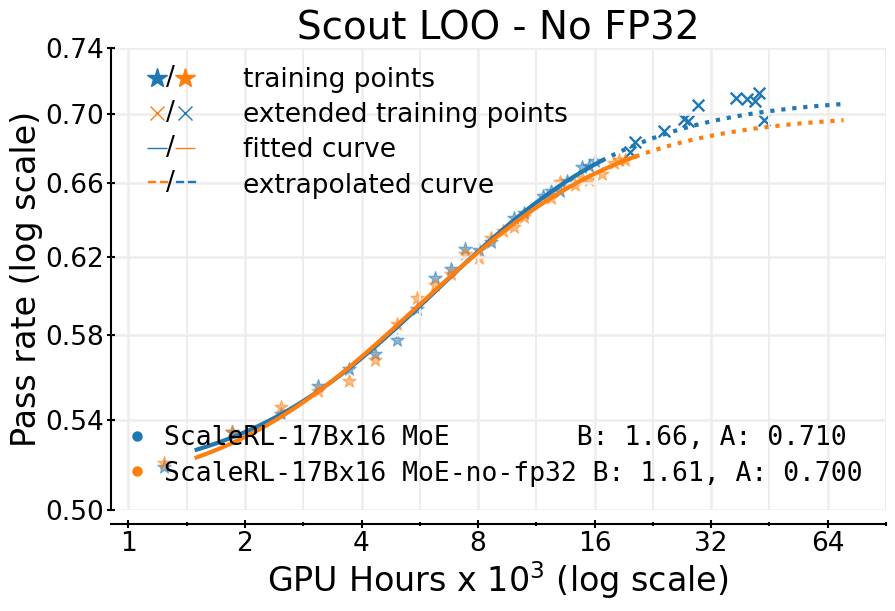
\includegraphics[width=0.49\textwidth]{paper_figs/scout_loo_fp32.png}\label{fig:scout_loo_fp32}}
    
    \caption{
    (a) \textbf{Variance in scaling fits}. We train 3 independent runs of \scalerl\ to measure variance. We observe a $\pm 0.02$ error margin for asymptotic performance $A$. (b) \textbf{FP32 LOO on Scout:} Comparing \scalerl\ on Scout with and without FP32 precision fix at the LM Head. \scalerl\ performs better with the FP32 fix.}
    \label{fig:scaling_and_error}
\end{figure*}


Across all axes, \scalerl\ consistently remains the most effective configuration, slightly outperforming LOO variants either in asymptotic reward or in compute efficiency (refer to the last column in the Figure~\ref{fig:LOO} table). Since most LOO variants reach similar asymptotic pass rates, we transform the sigmoidal fit to a power-law fit, to highlight efficiency differences via the slope $B$ (details in Figure~\ref{fig:LOO}). Concretely, we average the asymptotic reward $A$ across all runs, re-fit the curves with this fixed $A$, and then compare slopes (measuring efficiency) in Figure~\ref{fig:LOO}. The corresponding non-transformed pass-rate vs. compute curves are provided in Appendix~\ref{appendix:background}.

\paragraph{Error margin in fitting scaling curves} Since RL training is known to exhibit high variance~\citep{agarwal2021deep}, we use three independent \scalerl\ runs (\Cref{fig:error_margin}) to estimate the variability in fitted scaling coefficients. The observed variance in asymptotic reward and efficiency parameters serves as our empirical error margin, used to determine whether changes in compute efficiency or asymptotic performance are statistically meaningful for two different runs \citep{quantvar}.

\paragraph{Extrapolating Scaling Curves}
In all our LOO experiments as well as independent \scalerl\ runs, we fit the sigmoidal curve up to 8000 GPU-hours and extrapolate to 16000 GPU-hours, observing that the predicted curves align closely with both training and extended points. This demonstrates the stability and predictability of \scalerl\ and other stable, scalable recipes under large-scale RL training.

\paragraph{Are the design choices worth it?}
In \Cref{sec:fwd_ablations}, certain design choices alter asymptotic performance, such as loss type (\Cref{fig:loss_type}) and FP32 precision~(\Cref{fig:fp32}). However, in our LOO experiments with \scalerl\ ~(\Cref{fig:LOO}), these components appear less critical individually (last column in the figure). 
This raises the question of whether certain design choices can be safely left at their ``default'' values. 

We argue the answer is no. Even when a choice seems redundant in the combined recipe, it can still provide stability or robustness that can become decisive in other regimes. 
For example, while the FP32 precision fix makes little difference with dense 8B trained with \scalerl\ (\Cref{fig:LOO}), it provides large gains in GRPO/DAPO-style losses by mitigating numerical instabilities. This indicates that its benefits extend beyond the specific \scalerl\ configuration we study. To further test this, we ran a leave-one-out experiment on the Scout 17Bx16 MoE and observed that FP32 precision improves overall scalability (\Cref{fig:scout_loo_fp32}). 

A similar case arises with the loss type. In \Cref{fig:LOO}, reverting to DAPO yields similar asymptotic performance to CISPO within \scalerl. 
Nonetheless, as we discuss in Appendix~\ref{appendix:loss_types}, CISPO is markedly more robust to the choice of IS-clipping parameter $\epsilon_{\max}$, reducing the sensitivity of training to hyperparameter tuning. Moreover, it's also more efficient than DAPO, as seen in LOO experiment ($B=2.01$ vs $B=1.77$).
This justifies preferring CISPO, even if a carefully tuned DAPO variant can perform similar asymptotically. 

In summary, even when individual design choices appear redundant within the combined recipe, they often enhance training stability, robustness, or efficiency in ways that generalize across models and setups. \scalerl\ retains such components not just for marginal gains in a specific configuration, but because they address recurring sources of instability and variance that arise across reinforcement learning regimes.


\section{Predictable  Scaling Returns Across RL Compute Axes}\label{sec:diff_axes}

\begin{figure*}[t]
    \centering
    \subfloat[]{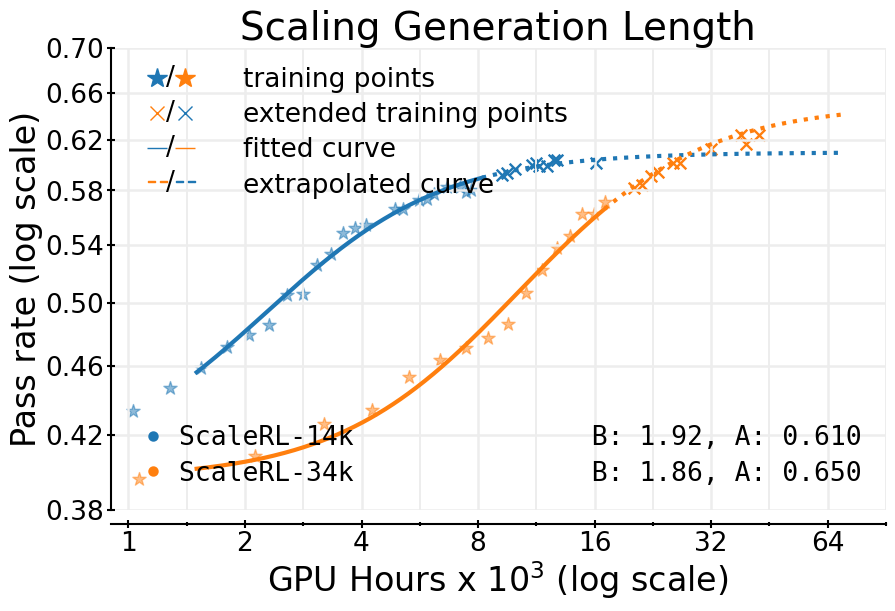
\includegraphics[width=0.50\textwidth]{paper_figs/large_scale_gen_len.png}}
    \hfill
    \subfloat[]{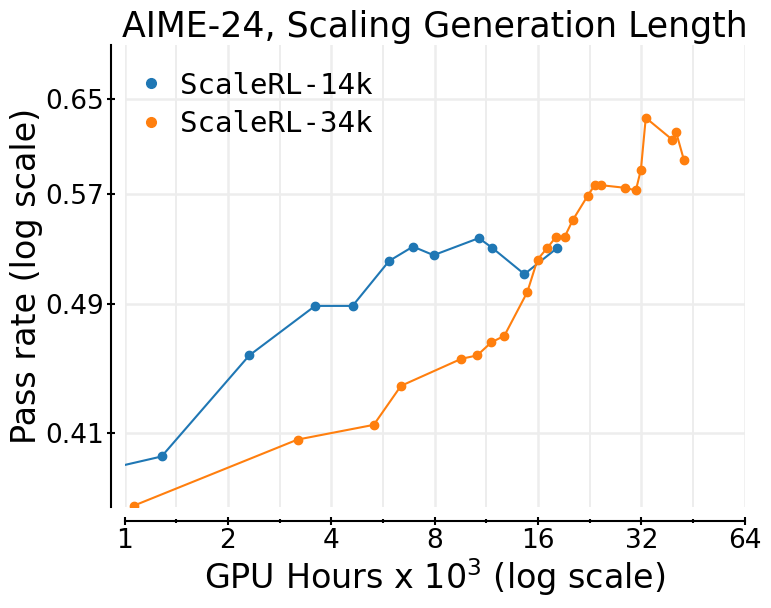
\includegraphics[width=0.44\textwidth]{paper_figs/large_scale_gen_len_aime24.png}}
    \hfill
    \caption{\small{\textbf{Scaling RL Generation Length}. While long-context RL is less efficient initially, it eventually surpasses the performance of the smaller-context run. This trend is observed on both the \emph{iid} validation set (left) as well as downstream evaluations (right).} 
    % {\color{red} Chop to same amount of compute on both plots, maybe 50K?}
    }
    \label{fig:large_scale_gen_len}
\end{figure*}


Given a fixed or growing compute budget, which scaling knob --context length, batch size, generations per prompt, and model size -- buys the most reliable performance gain, and how early can we predict that return? We answer this by (i) fitting the saturating power-law in \cref{eq:sigmoid_law} early in training for each setting (precisely, half the target budget), (ii) extrapolating to the target budget, and (iii) extending training to verify the forecast. Across all axes below we observe clean, predictive fits whose extrapolated curves align with the extended trajectories, mirroring the behavior seen in our 100,000 GPU-hour run (\Cref{fig_100k_main}), and the cross-recipe comparison in \Cref{fig:prevelant_methods}.


\paragraph{Model scale (MoE)}
Does ScaleRL remain predictive and stable on larger models? Training the 17B×16 Llama-4 Scout MoE with ScaleRL exhibits the same predictable scaling behavior as the 8B model, with low truncation rates and no instability pathologies (Appendix~\ref{appendix:truncations}, \ref{appendix:loss_types}). \Cref{fig_100k_main} shows the training curve. The extended points align with the fitted curve, supporting the model-scale invariance of our recipe. Moreover, the larger 17B×16 MoE exhibits much higher asymptotic RL performance than the 8B dense model, outperforming the 8B's performance using only $1/6$ of its RL training compute.

\paragraph{Generation length (context budget)}
Increasing the generation length from 14k to 32k tokens slows early progress (lower $B$ and higher $C_{mid}$) but consistently lifts the fitted asymptote (A), yielding higher final performance once sufficient compute is provided (\Cref{fig:large_scale_gen_len}). This validates long-context RL as a ceiling-raising knob rather than a mere efficiency trade-off. Extrapolations made from the fit correctly forecast the higher 32k-token trajectory when training is extended. 

\paragraph{Global batch size (prompts)} Smaller-batch runs show early stagnation on downstream benchmarks even as in-distribution validation performance continues to improve. Larger batches reliably improve the asymptote and avoid the downstream stagnation we observe in smaller-batch runs. \Cref{fig:large_scale_bsz} shows the same qualitative pattern at mid-scale: small batches may appear better early but are overtaken as compute grows. 
In our largest math run in \Cref{fig_100k_main}, moving to batch size of 2048 prompts both stabilized training and yielded a fit that extrapolated from up to 50k GPU hours to the final 100k point.

\paragraph{Generations per prompt (fixed total batch)}
For a fixed total batch, is it better to allocate more prompts or more generations per prompt? Sweeping generations per prompt {8,16,24,32} and adjusting prompts to keep total batch fixed leaves fitted scaling curves essentially unchanged (Appendix~\ref{appendix:large_scale}), suggesting that, at moderate batch, this allocation is a second-order choice for both A and B. Clearer differences may emerge at much larger batches (e.g., 2k+), which we leave for future work. 








\begin{figure*}[t!]
    \centering
    \subfloat[]{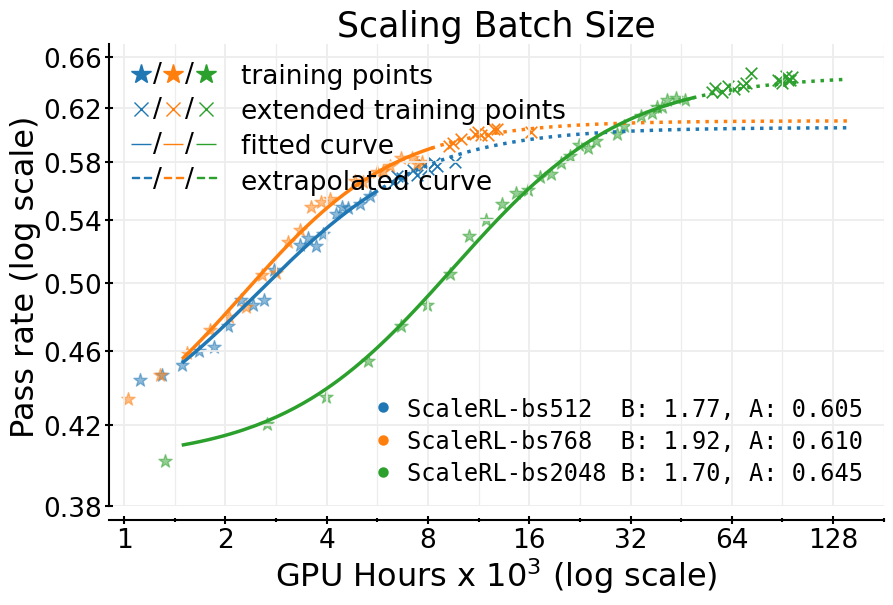
\includegraphics[width=0.48\textwidth]{paper_figs/large_scale_bsz.png} \label{fig:large_scale_bsz}}
    ~~
    \subfloat[]{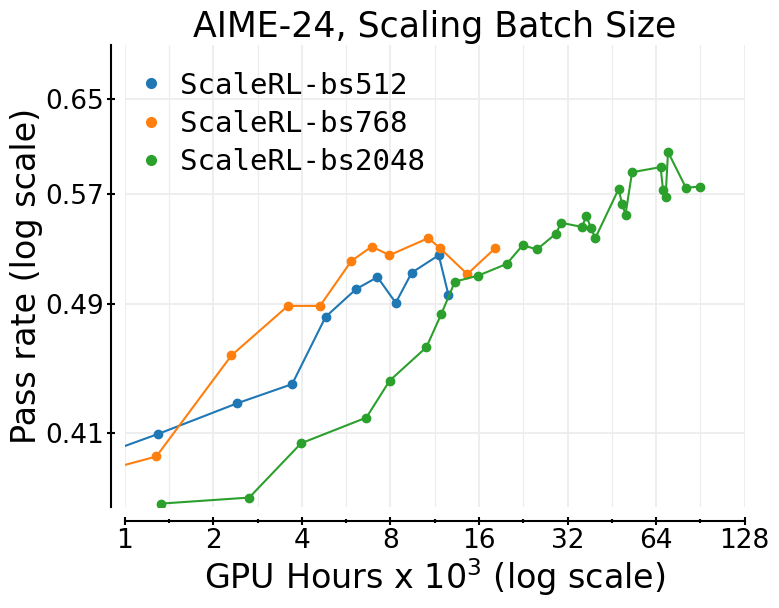
\includegraphics[width=0.4\textwidth]{paper_figs/large_scale_bsz_aime24.png} \label{fig:large_scale_bsz_aime24}}
    \caption{\small{\textbf{Scaling RL batch size}. larger batch size is slower in training but settles at a higher asymptote. Batch size show an inverse trend initially where smaller values seem better at lower compute budget, but reach a higher asymptotic performance at larger scale.} 
    }
\end{figure*}